\chapter{Fonctionnement général du système et les composantes électroniques}
\phantomsection
\addcontentsline{toc}{chapter}{Fonctionnement général du système}

\section{Fonctionnement général du système }
\subsection{Introduction}

Dans le chapitre précédent, le fonctionnement général d'un système solaire et les principaux paramètres d'une batterie ont été abordés. Ce nouveau chapitre se penche sur la conception et la réalisation du système de suivi en temps réel des batteries solaires. Seront détaillés les choix technologiques effectués, ainsi que les solutions adoptées pour la mesure et la surveillance des paramètres critiques tels que la tension, le courant, la température et l'état de charge et décharge des batteries.


\subsubsection{Présentation générale du dispositif}
Le dispositif est conçu pour surveiller en temps réel les paramètres essentiels des batteries solaires utilisées dans une installation photovoltaïque. Ce système capture des données telles que la tension, le courant et la température de chaque batterie individuellement, que les batteries soient montées en série ou en parallèle. Il fournit également des informations sur l'état de charge (SoC) et l'état de décharge (DoD) du système. En cas d'anomalie, le dispositif peut envoyer une alerte par SMS ou par email via l'application web, grâce à l'utilisation d'un microcontrôleur.

\subsubsection{Analyse des besoins du dispositif}
Avant de concevoir le dispositif, il est essentiel de comprendre ses besoins spécifiques. Voici les exigences pour notre dispositif :

\begin{itemize}
	\item Informations sur les paramètres de chaque batterie :
	\begin{itemize}
		\item Tension
		\item Courant
		\item Température
	\end{itemize}
	\item Traitement des informations de chaque batterie et de l'ensemble du système
	\item Envoi des données vers un système de stockage en ligne
	\item Visualisation des données stockées
	\item Alertes en cas de dysfonctionnement de la batterie
	\item Isolation des batteries pour une meilleure précision des mesures.
\end{itemize}

\subsubsection{Architecture générale du système}

Pour bien visualiser notre système global, nous pouvons classer les besoins par plusieurs blocs fonctionnels.

\begin{figure}[H]
	\centering
	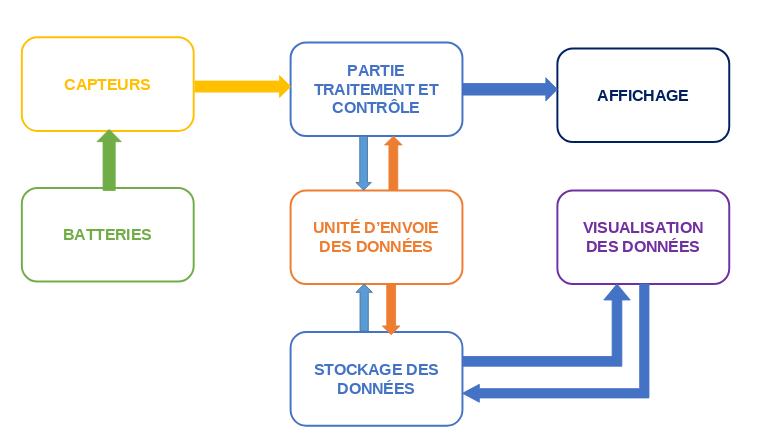
\includegraphics[width=17cm]{./img/schemaBloc.png}
	\caption{Schéma bloc du système général}
	\label{i1}
\end{figure}

Le système est composé de sept blocs distincts avec des fonctions précises. Nous allons détailler le fonctionnement de chaque bloc :

\paragraph{Bloc batterie :}
ce module est composé de trois batteries que le dispositif doit surveiller en temps réel.
\paragraph{Bloc des capteurs :}
cette section fournit les informations au reste du système. Elle est équipée des capteurs suivants :
\begin{itemize}
	\item Capteur de tension : mesure la tension de chaque batterie.
	\item Capteur de courant : mesure le courant de charge et de décharge de chaque batterie.
	\item Capteur de température :  évalue la température de chaque batterie. 
\end{itemize}

\paragraph{Unité de traitement et contrôle :}
cette partie constitue le cœur du dispositif. Elle analyse les données reçues des capteurs, effectue les calculs nécessaires, convertit les signaux analogiques en données exploitables par le système et héberge les programmes de contrôle.

\paragraph{Bloc d'affichage :}
cet élément est chargé de présenter les informations traitées par l'unité de contrôle de manière claire et accessible.

\paragraph{Unité d'envoi de données :}
il s’occupe de la communication des données traitées, selon les instructions de l'unité de traitement.

\paragraph{Centre de stockage :}
cette partie stocke les informations pré-traitées pour qu'elles puissent être utilisées pour surveiller l'état des batteries. Le stockage permet également de conserver un historique des données pour des analyses ultérieures.

\paragraph{Bloc de visualisation de données :}
ce bloc permet de visualiser les données en temps réel stockées par le centre de stockage.

\subsection{Principe de fonctionnement du dispositif}

Le but de ce dispositif est de surveiller en continu l'état de chaque batterie ainsi que celui de l'ensemble du système photovoltaïque.

La collecte des données sur les batteries se fait en deux étapes :

\begin{itemize} \item \textbf{Étape 1 :} mesure globale des batteries.
	À ce stade, nous collectons les données de tension, courant et température du système complet pour obtenir une vue d'ensemble du fonctionnement.
\item \textbf{Étape 2 :} mesure individuelle des batteries.  
Ici, chaque batterie est isolée pour effectuer des mesures précises de tension et de courant. Si cette opération se déroule pendant l'ensoleillement,il est possible de déconnecter le régulateur de charge afin d'éviter qu'il n'influence les valeurs mesurées par les capteurs. Nous procédons ainsi en séquence, en isolant chaque batterie l’une après l’autre, afin de déterminer leur état de fonctionnement et d'identifier celles qui nécessitent un remplacement.
\end{itemize}

\subsubsection{Organigramme}

Cet organigramme illustre la procédure logique à suivre pour assurer le bon fonctionnement de notre dispositif, en détaillant les étapes essentielles du processus de commande, de contrôle et d’exécution.



\begin{figure}[H]
	\centering
	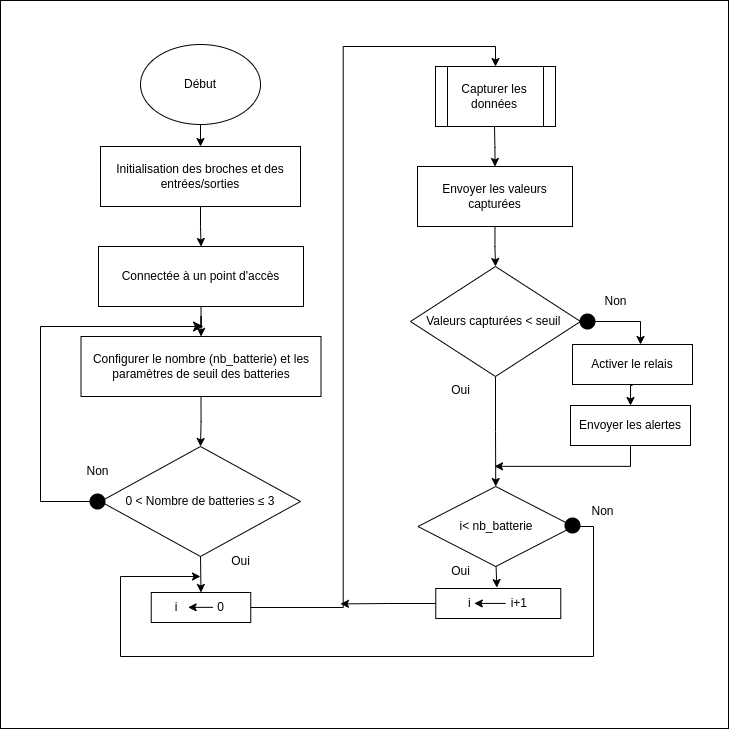
\includegraphics[width=15cm]{./img/organigramme.png}
	\caption{Organigramme du fonctionnement}
	\label{i1}
\end{figure}



\subsubsection{Étude d'une cas d'installation}

Pour nos étude on va prendre le cas d'une installation photovoltaïque qui à une puissance de 12Kw avec un tension de 400V.
On a vue dans le chapitre précèdent les procéder de dimensionnement d'une centrale photovoltaïque alors on va suivre ces étapes pour ce cas .


\subsubsection*{1. Besoin Énergétique des applications}
Supposons que les applications nécessitent une énergie totale de 12 kW en puissance crête.

\subsubsection*{2. Énergie solaire récupérable}
\begin{itemize}
	\item \textbf{Inclinaison et orientation des panneaux:}
	\begin{itemize}
		\item \textbf{Orientation:} les panneaux doivent être orientés vers le nord dans l'hémisphère sud pour maximiser la production.
		\item \textbf{Inclinaison:} pour Madagascar, une inclinaison égale à la latitude (environ 12°) est souvent recommandée \cite{pdf1}.
	\end{itemize}
	\item \textbf{Données météorologiques:} 
	supposons une irradiation moyenne de 5 kWh/m²/jour pour la période la moins ensoleillée.
\end{itemize}



%\begin{landscape}

\begin{table}[H]
	\centering
	\begin{tabular}{|>{\centering\arraybackslash}m{5cm}|>{\centering\arraybackslash}m{5cm}|>{\centering\arraybackslash}m{5cm}|}
		\hline
		\textbf{Calcul} & \textbf{Formule} & \textbf{Résultat} \\
		\hline
		\textbf{Énergie produite (Wh/jour)} & $E_p = \frac{E_c}{k}$ & $E_p = 17,143$ \text{ Wh/jour} \\
		\hline
		\textbf{Puissance crête } & $P_c = \frac{E_p}{Ir}$ & $P_c = 3,429$ \text{ W} \\
		\hline
		\textbf{Nombre de modules } & $N_p = \frac{P_c}{P_{pv}}$ & $N_p = 40$ \text{ modules} \\
		\hline
		\textbf{Nombre de panneaux en série } & $N_s = \frac{U}{V_m}$ & $N_s = 10$ \\
		\hline
		\textbf{Nombre de branches en parallèle } & $N_{bp} = \frac{N_p}{N_s}$ & $N_{bp} = 4$ \\
		\hline
		\textbf{Puissance crête d’un champ} & $P_{c/champ} = N_{bp} \times N_s \times P_{pv}$ & $P_{c/champ} = 12000$ \text{ W} \\
		\hline
		\textbf{Surface du générateur } & $S_t = S_m \times N_m$ & $S_t = 64$ \text{ m²} \\
		\hline
		\textbf{Capacité de batterie} & $C_j = \frac{E_c}{U}$ & $C_j = 30$ \text{ Ah/jour} \\
		\hline
		\textbf{Capacité totale des batteries} & $C_u = \frac{C_j \times N_j}{U \times P_d}$ & $C_u = 187,5$ \text{ Ah} \\
		\hline
		\textbf{Nombre de batteries} & $N_t = N_s \times N_p$ & $N_t = 18$ \text{ batteries} \\
		\hline
		\textbf{Courant maximal régulateur} & $I_{\text{max}} = \frac{P_{c/champ}}{U}$ & $I_{\text{max}} = 30$ \text{ A} \\
		\hline
		\textbf{Courant de sortie d’un panneau} & $I = \frac{P}{U}$ & $I = 7,5$ \text{ A} \\
		\hline
		\textbf{Section des câbles } & $S = \frac{\rho \cdot L}{R}$ & $S \approx 10$ \text{ mm²} \\
		\hline
		\textbf{Courant circulant entre batteries et onduleur} & $I_{\text{max batteries}} = \frac{P_{\text{max onduleur}}}{U_{\text{batterie}}}$ & $I_{\text{max batteries}} = 30$ \text{ A} \\
		\hline
	\end{tabular}
	\caption{Résumé des calculs pour le dimensionnement du système photovoltaïque}
	\label{tab:calculs_dimensionnement}
\end{table}
%\end{landscape}

\section{Les composantes électroniques adaptés au projet}

Selon le schéma bloc du système et les principes de fonctionnement décrits précédemment, plusieurs composants électroniques sont nécessaires pour réaliser le dispositif. Pour cette étude, nous prenons comme référence un dispositif capable de supporter une puissance maximale de 12 kW à la sortie de l'onduleur, avec une tension de 400 V et un courant de 30 A à l'entrée. Les composants requis pour cette configuration sont les suivants :

\subsection{Les capteurs et instruments de Mesure}

Des capteurs sont nécessaires pour surveiller le système et collecter des données pour le contrôle :

\subsubsection{Les capteurs de courant et de tension }
\subsubsection*{Pour le courant : modules ACS712 30A}

Le ACS712 utilise la technologie de l'effet Hall pour détecter le courant passant à travers le conducteur mesuré. L'effet Hall est un phénomène où une tension est générée perpendiculairement au flux de courant dans un matériau conducteur lorsqu'il est soumis à un champ magnétique  \cite{1}.

Il est conçu pour mesurer à la fois les courants AC et DC avec une grande précision, et sa sortie est un signal analogique qui varie en fonction de l'intensité du courant mesuré.


\begin{figure}[H]
	\centering
	\begin{subfigure}{0.40\textwidth} % Largeur de la première image
		\centering
		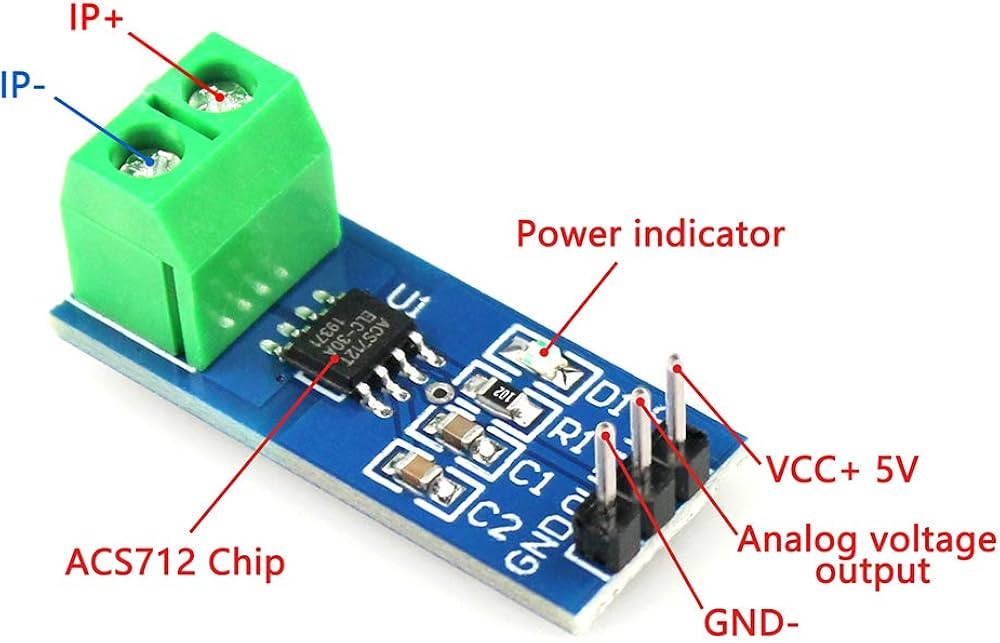
\includegraphics[width=\linewidth]{./img/composants/ACS712.jpg}
		\label{fig:acs712a}
	\end{subfigure}
	\hfill
	\begin{subfigure}{0.55\textwidth} % Largeur de la deuxième image
		\centering
		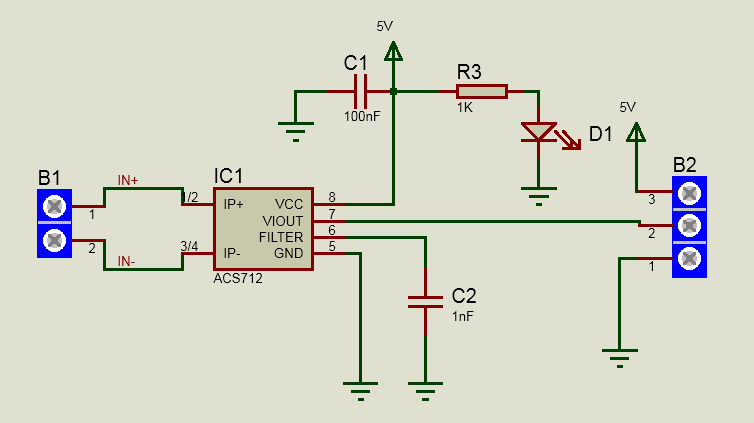
\includegraphics[width=\linewidth]{./img/composants/ACS.PNG}
		\label{fig:acs712b}
	\end{subfigure}
	\caption{Modules ACS712 30A  \cite{1} et son schéma}
	\label{fig:combined}
\end{figure}
\subsubsection*{Caractéristiques techniques }

\begin{itemize}
	\item \textbf{Plage de mesure du courant :} 
	\begin{itemize}
		\item De -30A à +30A (AC ou DC)
	\end{itemize}
	
	\item \textbf{Sensibilité (pour le modèle 30A) :}
	\begin{itemize}
		\item 66 mV par ampère (66 mV/A)
	\end{itemize}
	
	\item \textbf{Type de capteur :}
	\begin{itemize}
		\item Effet Hall (non-intrusif, sans contact direct avec le conducteur)
	\end{itemize}
	
	\item \textbf{Tension d'alimentation :} 
	\begin{itemize}
		\item 5V DC
	\end{itemize}
	
	\item \textbf{Tension de sortie :} 
	\begin{itemize}
		\item La tension de sortie du capteur est proportionnelle au courant mesuré. Lorsque le courant est nul, la sortie est à 2,5V (milieu de la plage d'alimentation). Les variations de courant font monter ou descendre cette tension :
		\begin{itemize}
			\item 0A $\rightarrow$ environ 2,5V
			\item Courant positif (jusqu’à 30A) $\rightarrow$ sortie augmente à partir de 2,5V
			\item Courant négatif (jusqu’à -30A) $\rightarrow$ sortie diminue à partir de 2,5V
		\end{itemize}
	\end{itemize}
	
	\item \textbf{Précision :}
	\begin{itemize}
		\item Erreur typique de ±1,5\%
	\end{itemize}
	
	\item \textbf{Tension d'isolation :}
	\begin{itemize}
		\item 2,1 kV RMS (entre la partie du circuit de puissance et la partie de mesure)
	\end{itemize}
	
	\item \textbf{Impédance interne (entrée) :}
	\begin{itemize}
		\item Très faible, donc une chute de tension négligeable à travers le capteur.
	\end{itemize}
	
	\item \textbf{Temps de réponse :}
	\begin{itemize}
		\item Typiquement 5 $\mu$s (rapide pour des mesures de courant dynamique)
	\end{itemize}
	
	\item \textbf{Largeur de bande :}
	\begin{itemize}
		\item 80 kHz
	\end{itemize}
	
	\item \textbf{Type de signal de sortie :}
	\begin{itemize}
		\item Analogique (à connecter à une entrée analogique d'un microcontrôleur ou d'une carte d'acquisition de données)
	\end{itemize}
\end{itemize}


\subsubsection*{Pour la tension : diviseur de tension}

Un diviseur de tension est un circuit simple constitué de deux résistances connectées en série, utilisé pour réduire la tension d'entrée à une valeur proportionnelle à la tension souhaitée. Ce type de circuit est souvent utilisé pour mesurer des tensions élevées, comme celles des batteries solaires, et les adapter à la plage de mesure des capteurs ou des microcontrôleurs.

\begin{figure}[H]
	\centering
	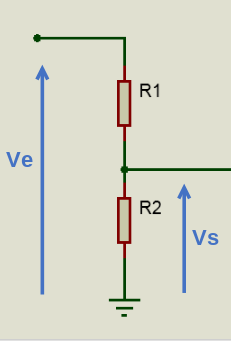
\includegraphics[width=3cm]{./img/composants/DDT.png}
	\caption{Schéma d'un diviseur de tension }
	\label{i1}
\end{figure}



\subsubsection*{Caractéristiques techniques}

\textbf{Tension d'entrée (Ve)} :
\begin{itemize}
	\item La tension de la batterie solaire (par exemple, 12V, 24V ou 48V) est appliquée au point d'entrée du diviseur de tension.
	\item La tension d'entrée maximale dépend des résistances sélectionnées et de la capacité des composants à dissiper la puissance.
\end{itemize}

\textbf{Tension de sortie (Vs)} :
\begin{itemize}
	\item La tension de sortie est proportionnelle à la tension d'entrée selon la formule :
	\begin{equation}
		V_{s} = V_{e} \times \frac{R2}{R1 + R2}
	\end{equation}
	\item Cette sortie est souvent adaptée à une tension de 5V ou 3.3V pour être compatible avec les entrées analogiques des microcontrôleurs comme l'Arduino ou l'ESP32.
\end{itemize}

\textbf{Précision} :
\begin{itemize}
	\item La précision dépend de la tolérance des résistances. Utiliser des résistances avec une faible tolérance (1\% ou moins) améliore la précision du diviseur.
\end{itemize}

\textbf{Puissance dissipée} :
\begin{itemize}
	\item Les résistances doivent être choisies en fonction de leur capacité à dissiper la chaleur. La puissance dissipée par chaque résistance est calculée comme :

	
	\begin{equation}
		P = \frac{V^2}{R}
	\end{equation}
\end{itemize}

\subsubsection{Capteurs de température LM35}
Le LM35 est un capteur de température de précision dont la sortie est proportionnelle à la température ambiante mesurée. Le LM35 produit une sortie en tension linéaire avec la température en degrés Celsius, ce qui le rend facile à utiliser avec les microcontrôleurs et les systèmes de mesure analogiques sans avoir besoin de conversion de température  \cite{3}.

\begin{figure}[H]
	\centering
	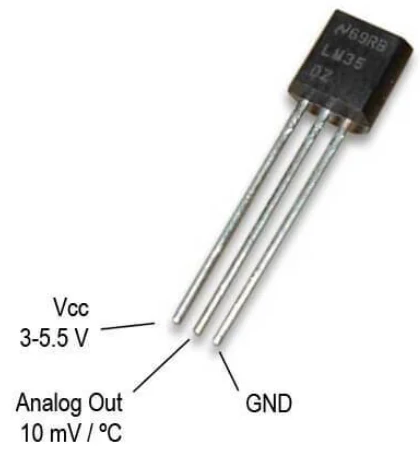
\includegraphics[width=4cm]{./img/composants/LM35.png}
	\caption{Le capteur LM35}
	\label{i1}
\end{figure}

\subsubsection*{Caractéristiques Techniques du LM35}
\begin{itemize}
	\item \textbf{Plage de température mesurable} : -55°C à +150°C
	\item \textbf{Précision} : 
	\begin{itemize}
		\item ±0.5°C à 25°C
		\item ±0.75°C sur la plage complète
	\end{itemize}
	\item \textbf{Tension de sortie} : 10 mV/°C
	\item \textbf{Tension d'alimentation} : 4V à 30V
	\item \textbf{Courant d'alimentation} : Typiquement 60 µA
	\item \textbf{Impédance de sortie} : $\ 0.1 \Omega $ (pour un courant de sortie jusqu’à 1 mA)
	\item \textbf{Temps de réponse} : 1 seconde (pour 63\% de variation)
	\item \textbf{Linéarité} : Sortie linéaire par rapport à la température
	\item \textbf{Compatibilité} : Compatible avec les entrées analogiques des microcontrôleurs
\end{itemize}

\subsection{Partie traitement et contrôle}
\subsubsection{Microcontrôleur ESP 32 WROOM 32}
\textbf{Déscription}

Suite au succès de l'ESP8266, l'ESP32 a été introduit, offrant des performances nettement supérieures à son prédécesseur. L'ESP32 est une série de microcontrôleurs SoC (System on Chip) développée par Espressif Systems, reposant sur l'architecture Xtensa LX6 de Tensilica, avec des fonctionnalités intégrées pour le Wi-Fi et le Bluetooth. Parmi les outils de développement disponibles, on retrouve l'Arduino IDE, un logiciel libre conçu en C++, qui inclut un grand nombre de bibliothèques, ainsi que de nombreuses bibliothèques tierces dédiées aux applications embarquées et temps réel  \cite{5}.\\

\textbf{La structure externe et structure interne }\\
Voici les structures externe et interne du microcontrôleur ESP32 présentées ci-dessous :
\begin{figure}[H]
	\centering
	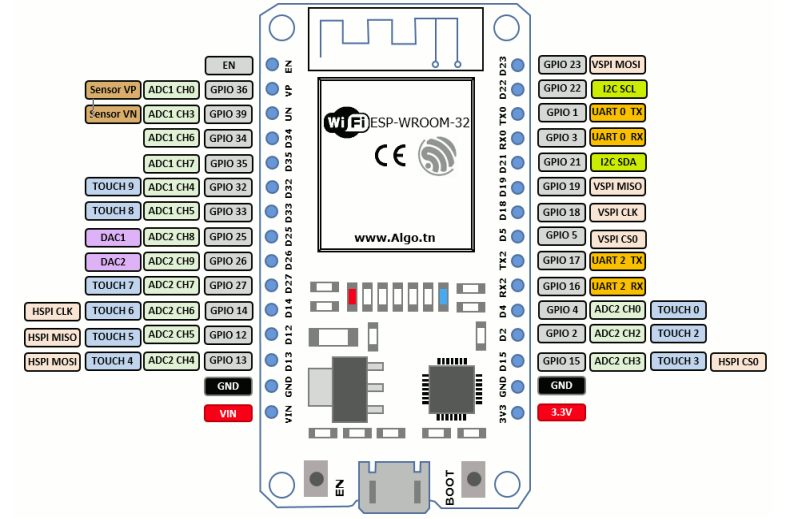
\includegraphics[width=15cm]{./img/composants/esp.png}
	\caption{La structure externe  \cite{8} }
	\label{i1}
\end{figure}



\begin{figure}[H]
	\centering
	\begin{subfigure}{0.40\textwidth} % Largeur de la première image
		\centering
		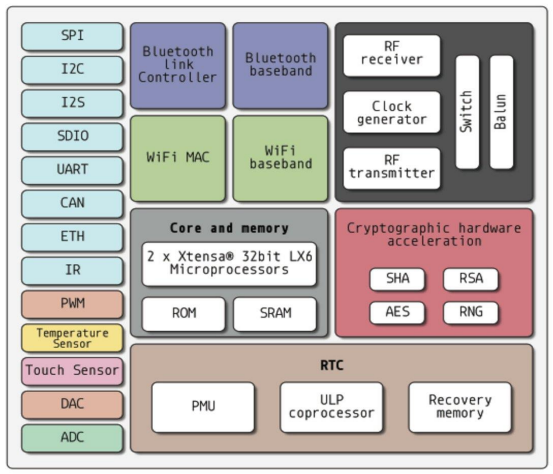
\includegraphics[width=9cm]{./img/composants/espInterne.png}
		\caption{La structure interne \cite{8} }
		\label{i1}
	\end{subfigure}
	\hfill
	\begin{subfigure}{0.55\textwidth} % Largeur de la deuxième image
			\centering
		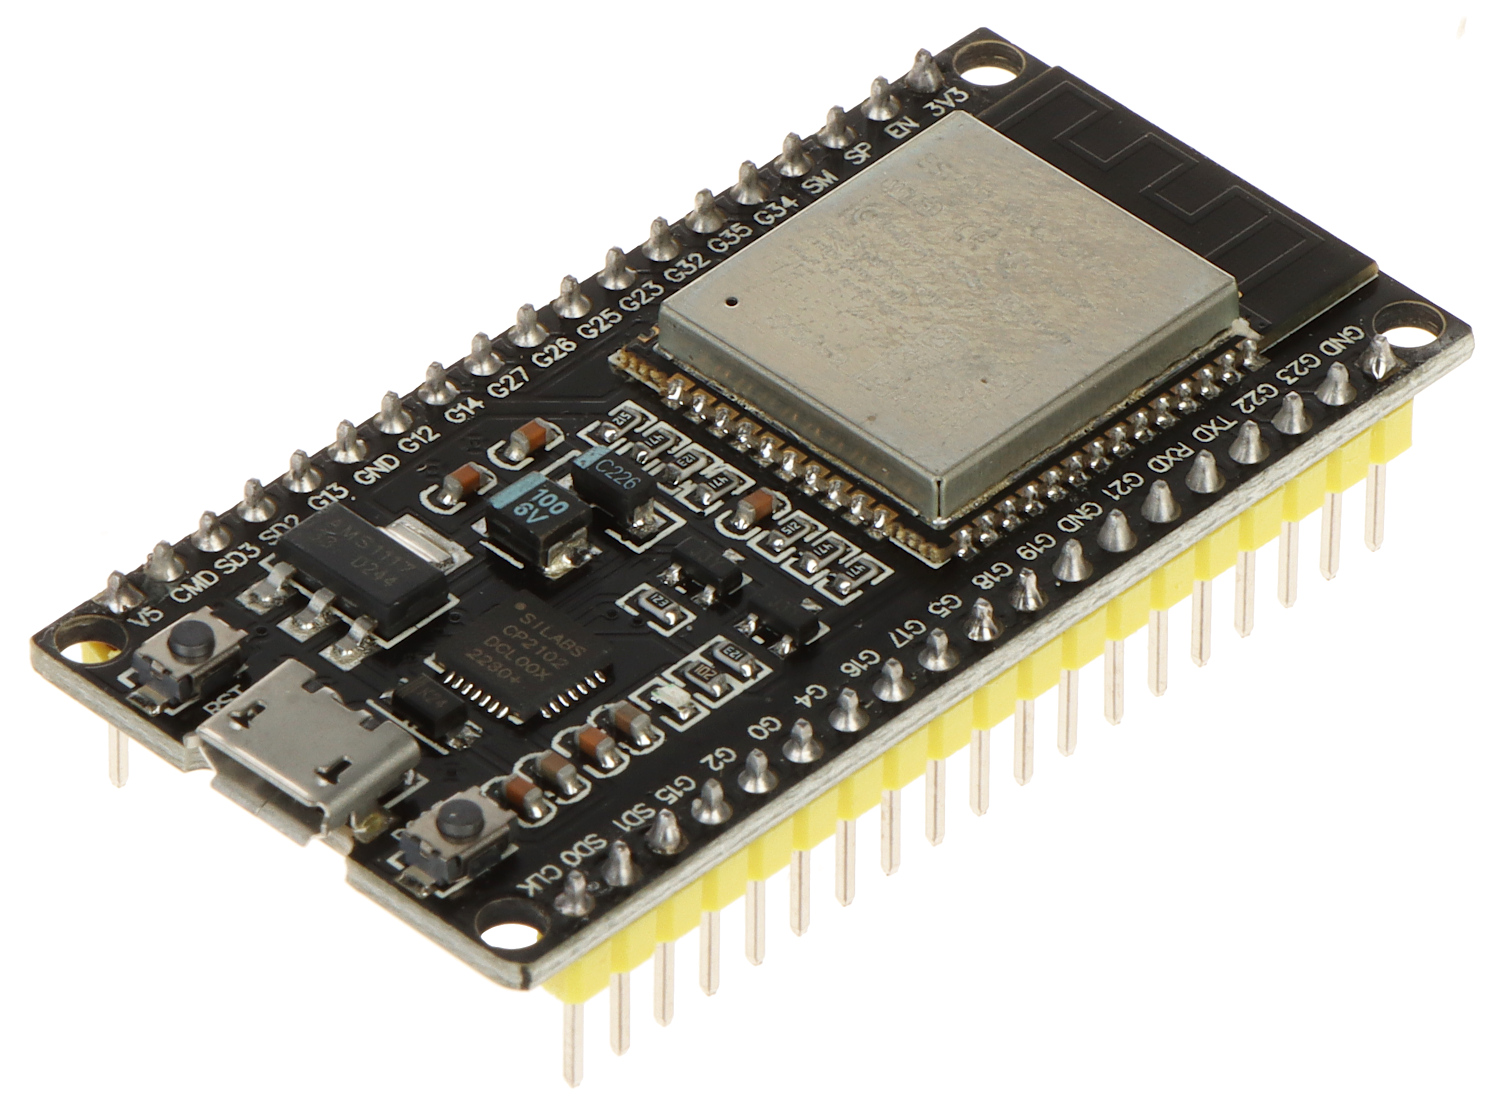
\includegraphics[width=5cm]{./img/composants/ESP.jpg}
		\caption{L'ESP 32 WROOM 32  \cite{5} }
		\label{i1}
	\end{subfigure}
\end{figure}

\subsubsection*{Ses principales spécifications techniques sont les suivantes :}

\begin{itemize}
	\item \textbf{Processeur :} microprocesseur Xtensa double cœur 32 bits, fonctionnant à 160 ou 240 MHz, offrant jusqu'à 600 MIPS.
	\item \textbf{Mémoire :}
	\begin{itemize}
		\item ROM : 448 Ko
		\item Flash : 4 Mo
		\item RAM : 520 Ko de SRAM
	\end{itemize}
	\item \textbf{Ressources :}
	\begin{itemize}
		\item Broches : 32 GPIO avec ADC (12), DAC (2), SPI (3), I2S (2), I2C (2), UART (3), PWM (32), SDIO (50 MHz)
		\item Connectivité sans fil :
		\begin{itemize}
			\item Wi-Fi : 802.11 b/g/n à 2,4 GHz, avec un débit maximal de 150 Mbps
			\item Bluetooth
		\end{itemize}
		\item Contrôleur infrarouge intégré
		\item Capteur à effet Hall
		\item Préamplificateur analogique intégré
	\end{itemize}
	\item \textbf{Consommation énergétique :} Très faible
	\item \textbf{Plage de température de fonctionnement :} -40°C à 125°C
	\item \textbf{Tension d'alimentation :} 2,2V à 3,6V DC
\end{itemize}


Le ESP32 est choisi pour sa capacité à gérer les communications sans fil et son support pour de multiples interfaces de capteurs et actuateurs, ce qui le rend idéal pour les applications IoT dans un système photovoltaïque.

\subsection{Afficheur LCD avec module I2C}
Le module LCD 2x16 est un écran à cristaux liquides qui peut afficher deux lignes de 16 caractères chacune. Lorsqu'il est combiné avec un module I2C, il permet de contrôler l'écran avec seulement deux fils pour la communication (SDA et SCL) en plus de l'alimentation. Cela simplifie grandement les connexions et le câblage, rendant le LCD plus facile à utiliser avec des microcontrôleurs  \cite{6}.
\begin{figure}[H]
	\centering
	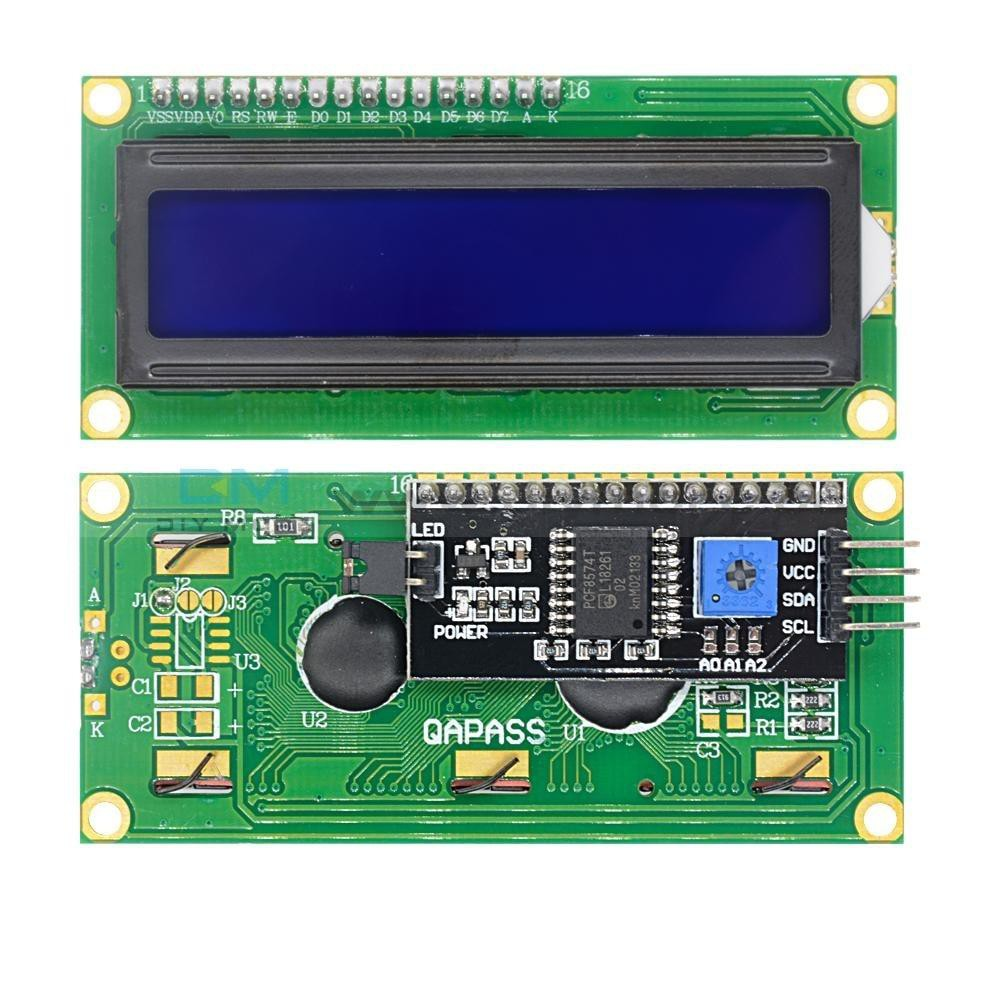
\includegraphics[width=6cm]{./img/composants/lcdI2C.jpeg}
	\caption{Le LCD 2x16 avec module I2C  \cite{6}}
	\label{i1}
\end{figure}
\subsubsection*{Caractéristiques du LCD 2x16 avec I2C}

\begin{itemize}[label={--}]
	\item \textbf{Dimensions de l'écran} : 2 lignes x 16 caractères.
	\item \textbf{Type de module} : LCD 16x2 avec interface I2C.
	\item \textbf{Affichage} : LCD à rétroéclairage LED
	\item \textbf{Interface I2C} : Communication via SDA (données) et SCL (horloge).
	\item \textbf{Alimentation} : 5V
	\item \textbf{Adresse I2C} : Souvent 0x27 ou 0x3F.
	\item \textbf{Commandes et fonctionnalités} : commandes LCD standards, affichage de texte et caractères spéciaux.
	\item \textbf{Consommation d'énergie} : faible, adapté aux projets alimentés par batterie.
	\item \textbf{Connectivité} : 4 broches (VCC, GND, SDA, SCL).
\end{itemize}

\subsection{Module de Communication}

Le module de communication permet d’envoyer les données collectées vers une plateforme en ligne, facilitant le suivi à distance. Le module GSM SIM900 est utilisé pour sa compatibilité avec les réseaux GSM/GPRS.\\

\textbf{Module GSM SIM900 :} Utilisé dans les applications IoT pour la communication sans fil, ce module permet la transmission de données par SMS ou GPRS.

\begin{itemize} \item \textbf{Caractéristiques techniques :}
	
	\begin{itemize}
		\item \textbf{Fréquences GSM :} quadri-bande (850, 900, 1800, 1900 MHz), compatible avec la plupart des réseaux mondiaux.
		
		\item \textbf{Interface UART :} communication avec microcontrôleurs via UART, configurable jusqu'à 115200 bps. Commandes AT pour gérer les SMS et la transmission de données (`AT+CMGF`, `AT+CMGS`).
		
		\item \textbf{GPRS classe 10 :} débit maximal de 85.6 kbps pour la transmission de données TCP/IP. Compatible avec les protocoles HTTP et FTP pour l'envoi de données à un serveur distant.
		
		\item \textbf{Alimentation :} fonctionne entre 3.2V et 4.8V, avec une consommation de 1.5 mA en veille et jusqu’à 2A lors des pics de transmission.
		
		\item \textbf{Mode d’économie d’énergie :} mode veille (1.5 mA) pour prolonger l’autonomie dans les applications à basse consommation.
	\end{itemize}
	
	\begin{figure}[H]
		\centering
		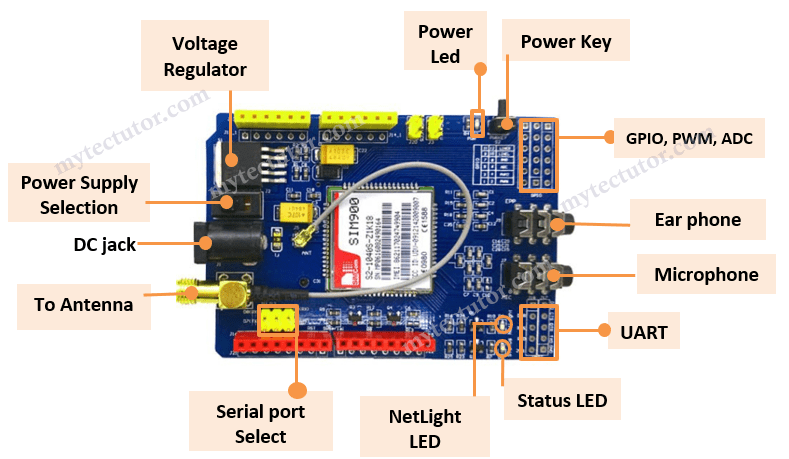
\includegraphics[width=12cm]{./img/composants/SIM900.png}
		\caption{Le module GSM SIM900 \cite{7}}
		\label{i1}
	\end{figure}
	
	\item \textbf{Avantages :}
	\begin{itemize}
		\item \textbf{Fiabilité :} adapté aux environnements éloignés grâce à la couverture GSM étendue.
		\item \textbf{Faible coût :} rentable pour les projets IoT nécessitant une connectivité cellulaire.
		\item \textbf{Compatibilité :} facile à intégrer avec des microcontrôleurs via UART et commandes AT.
	\end{itemize}
	
	\item \textbf{Inconvénients :}
	\begin{itemize}
		\item \textbf{Débit limité :} GPRS offre un débit faible comparé aux technologies modernes (3G/4G).
		\item \textbf{Consommation d’énergie élevée :} pics de consommation jusqu’à 2A lors des transmissions GPRS.
	\end{itemize}
	
 \end{itemize}


\subsection{Module relais 5V DC}
\subsubsection*{Description}
Le module relais 5V DC permet de contrôler des charges à haute tension à l'aide de signaux de faible puissance provenant de microcontrôleurs ou autres circuits de commande. Grâce à son système d'isolation, il protège le circuit de commande contre les surtensions et interférences provenant du côté de la charge \cite{2}.

\subsubsection*{Caractéristiques}

\begin{itemize}[label={--}]
	\item \textbf{Type de relais} : Relais électromagnétique.
	\item \textbf{Tension de commande} : 5V DC.
	\item \textbf{Capacité de charge} : 
	\begin{itemize}[label={*}]
		\item \textbf{AC} : Jusqu'à 250V AC, 10A.
		\item \textbf{DC} : Jusqu'à 30V DC, 10A.
	\end{itemize}
	\item \textbf{Connectivité} :
	\begin{itemize}[label={*}]
		\item \textbf{Broches de contrôle} : IN1, IN2, etc. pour les signaux de commande.
		\item \textbf{Broches d'alimentation} : VCC, GND pour l'alimentation du module.
		\item \textbf{Broches de relais} : COM, NO (Normalement Ouvert), NC (Normalement Fermé) pour la connexion de la charge.
	\end{itemize}
	\item \textbf{Indicateur LED} : LEDs pour indiquer l'état de chaque relais.
	\item \textbf{Isolation} : isolation optique entre le circuit de commande et le circuit de charge, réalisée à l'aide d'un optocoupleur.
\end{itemize}

\subsubsection*{Isolation}
L'isolation protège le microcontrôleur contre les surtensions et interférences provenant du circuit de puissance. Le module relais utilise un \textbf{optocoupleur} (\textbf{PC817}) pour assurer une isolation galvanique, permettant de transmettre un signal sans connexion physique directe. Cela aide à :
\begin{itemize}[label={*}]
	\item \textbf{Protéger le microcontrôleur} des hautes tensions.
	\item \textbf{Réduire les interférences électromagnétiques.}
	\item \textbf{Assurer la sécurité électrique.}
\end{itemize}

\textbf{Fonctionnement de l'optocoupleur} : 
nn optocoupleur est un composant qui utilise une diode LED pour transmettre des signaux électriques à travers la lumière. Le côté commande active la LED interne de l'optocoupleur, qui est détectée par un phototransistor du côté relais. Ainsi, le microcontrôleur reste isolé de la partie haute tension du circuit.

%\begin{figure}[H]
%	\centering
%	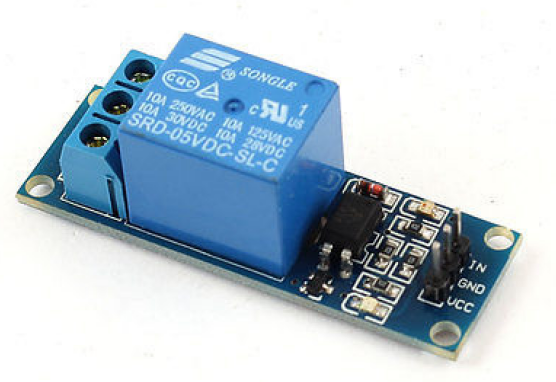
\includegraphics[width=6cm]{./img/composants/relais.png}
%	\caption{Module relais 5V DC}
%	\label{fig:relais_5vdc}
%\end{figure}
	
	
	
	\begin{figure}[H]
		\centering
		\begin{subfigure}{0.25\textwidth} % Largeur de la première image
			\centering
			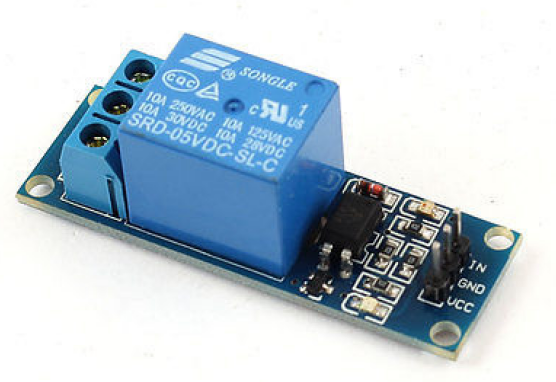
\includegraphics[width=\linewidth]{./img/composants/relais.png}
			\label{fig:acs712a}
		\end{subfigure}
		\hfill
		\begin{subfigure}{0.70\textwidth} % Largeur de la deuxième image
			\centering
			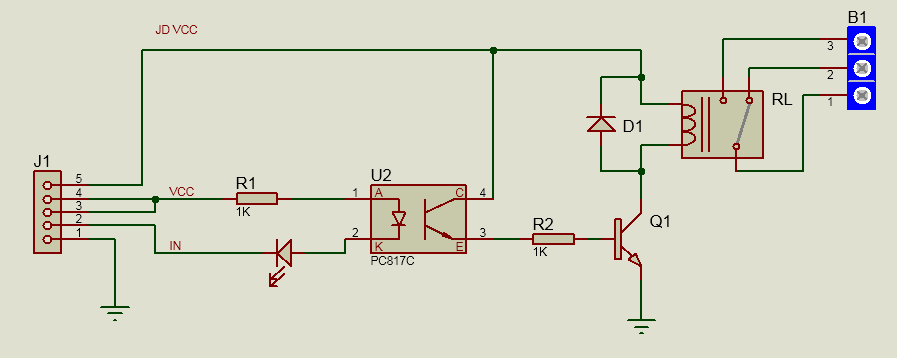
\includegraphics[width=12cm]{./img/composants/relais.PNG}
			\label{fig:acs712b}
		\end{subfigure}
		\caption{Module relais 5V DC \cite{2} et son schéma}
		\label{fig:combined}
	\end{figure}
	
\subsection{Transistor 2N2222}
	
	Pour éviter de surcharger le microcontrôleur, nous allons utiliser un transistor bipolaire en mode commutation. Un transistor nécessite seulement un faible courant pour atteindre l'état de saturation. Le modèle que nous choisirons est le 2N2222, un transistor bipolaire. Ses caractéristiques sont les suivantes \cite{9}:
	
\begin{itemize}[label={--}]
	\item \textbf{Type} : NPN
	\item \textbf{Tension maximale collecteur-émetteur} : 30 V
	\item \textbf{Courant continu collecteur} : 800 mA
	\item \textbf{Dissipation de puissance} : 500 mW
	\item \textbf{Fréquence de transition} : 250 MHz
	\item \textbf{Gain en courant DC (hFE min)} : 100
	\item \textbf{Plage de température de fonctionnement} : -65°C à +200°C
\end{itemize}
\begin{figure}[H]
	\centering
	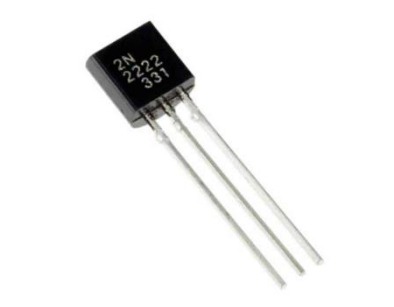
\includegraphics[width=6cm]{./img/composants/2n2222.png}
	\caption{Le transistor 2N2222}
	\label{fig:relais_5vdc}
\end{figure}
\subsection{Diode Zener 1N4728A}

\subsubsection*{Description}
La diode Zener 1N4728A est une diode à effet Zener conçue pour la régulation de tension et la protection contre les surtensions. Elle maintient une tension constante de 3.3V lorsqu'une tension plus élevée est appliquée dans la direction inverse, protégeant ainsi des composants sensibles comme l'ESP32 \cite{4}.

\subsubsection*{Caractéristiques}

\begin{itemize}[label={--}]
	\item \textbf{Type} : Diode Zener
	\item \textbf{Tension Zener} : 3.3 V (tension de régulation)
	\item \textbf{Courant Zener nominal} : 76mA
	\item \textbf{Puissance dissipée maximale} : 500 mW
	\item \textbf{Température de fonctionnement} : -65°C à +150°C
	\item \textbf{Tension inverse maximale} : 100 V
	\item \textbf{Tolérance de la tension Zener} : ±5\%
\end{itemize}
\begin{figure}[H]
	\centering
	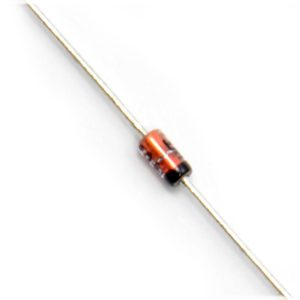
\includegraphics[width=4cm]{./img/composants/1n4728.jpg}
	\caption{Le diode zener 1N4728A}
	\label{fig:relais_5vdc}
\end{figure}
\section{Le système multi-capteurs contrôlé par ESP32}

Le dispositif de monitoring des batteries solaires est conçu pour capturer les paramètres clés des batteries et du système, tels que les tensions, les courants et les températures de chaque batterie. Pour mesurer les courants et les températures des batteries, le système utilise des capteurs ACS712 et LM35 respectivement. La tension des batteries est mesurée à l'aide d'un diviseur de tension qui réduit la tension à un niveau compatible avec les entrées analogiques de l'ESP32.

Pour garantir une mesure précise et efficace, chaque batterie est isolée par des relais. Les trois relais sont alternés pour activer et désactiver chaque batterie successivement. Un relais supplémentaire est connecté au régulateur de charge afin de l'isoler et obtenir des mesures fiables, que ce soit durant l'ensoleillement ou la nuit.

Les données capturées par les capteurs sont traitées par le microcontrôleur ESP32, qui est responsable de l'analyse, du traitement et de la commande des relais. Les informations traitées par l'ESP32 sont affichées sur un écran LCD et transmises à une base de données en ligne pour le stockage. L'ESP32 recueille également les paramètres configurés par l'utilisateur.

La transmission des données se fait principalement par Wi-Fi, grâce au module intégré de l'ESP32.

\begin{figure}[H]
	\centering
	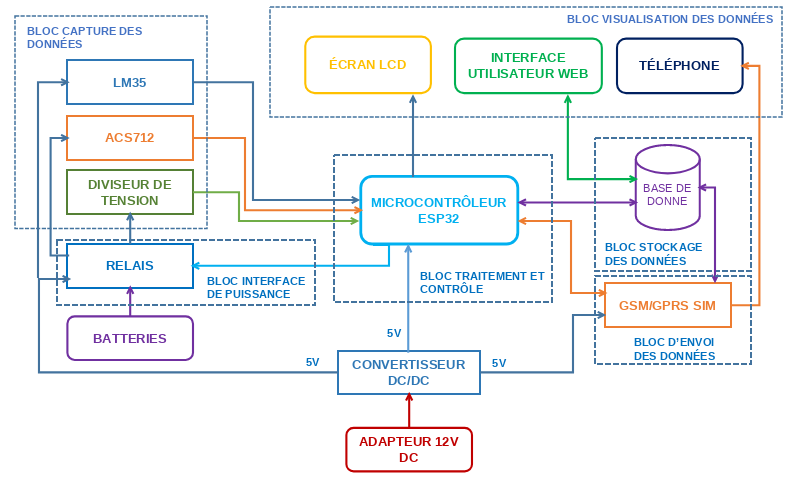
\includegraphics[width=17cm]{./img/composants/SCHEMAFONCTIONNEL.png}
	\caption{Le schéma fonctionnel}
	\label{fig:relais_5vdc}
\end{figure}


%\section{Étalonnage des capteurs}

%Afin d'assurer un fonctionnement optimal de nos capteurs de température, de courant et de tension, il est nécessaire de passer par des étapes d’étalonnage. Ce processus consiste à ajuster les capteurs afin de corriger les écarts de mesure et d'assurer des résultats précis.

%Dans notre projet, nous disposons de plusieurs capteurs : 4 capteurs ACS712 pour mesurer le courant, 4 diviseurs de tension pour mesurer la tension, et 3 capteurs LM35 pour mesurer la température. Pour garantir la précision des mesures, chaque capteur sera étalonné individuellement.

%\subsubsection{Étalonnage des capteurs ACS712}

%\textbf{Capteur ACS712 numéro 01 :}

%\begin{table}[H]
%	\centering
%	\begin{tabular}{|>{\centering\arraybackslash}m{4cm}|>{\centering\arraybackslash}m{3cm}|>{\centering\arraybackslash}m{3cm}|>{\centering\arraybackslash}m{3cm}|}
%		\hline
%		\textbf{Valeurs de l’étalon de référence (A)} & \textbf{Valeurs du capteur (A)} & \textbf{Écart de mesure (A)} & \textbf{Écart de mesure (\%)} \\
%		\hline
%		0.5 & 0.48 & -0.02 & -4.0 \\
%		1.0 & 0.98 & -0.02 & -2.0 \\
%		1.5 & 1.46 & -0.04 & -2.7 \\
%		2.0 & 1.98 & -0.02 & -1.0 \\
%		\hline
%	\end{tabular}
%	\caption{Étalonnage du capteur ACS712 numéro 01}
%	\label{tab:acs712_01}
%\end{table}

%\textbf{Capteur ACS712 numéro 02 :}

%\begin{table}[H]
%	\centering
%	\begin{tabular}{|>{\centering\arraybackslash}m{4cm}|>{\centering\arraybackslash}m{3cm}|>{\centering\arraybackslash}m{3cm}|>{\centering\arraybackslash}m{3cm}|}
%		\hline
%		\textbf{Valeurs de l’étalon de référence (A)} & \textbf{Valeurs du capteur (A)} & \textbf{Écart de mesure (A)} & \textbf{Écart de mesure (\%)} \\
%		\hline
%		0.5 & 0.49 & -0.01 & -2.0 \\
%		1.0 & 0.97 & -0.03 & -3.0 \\
%		1.5 & 1.47 & -0.03 & -2.0 \\
%		2.0 & 2.01 & +0.01 & +0.5 \\
%		\hline
%	\end{tabular}
%	\caption{Étalonnage du capteur ACS712 numéro 02}
%	\label{tab:acs712_02}
%\end{table}

%\textbf{Capteur ACS712 numéro 03 :}

%\begin{table}[H]
%%	\begin{tabular}{|>{\centering\arraybackslash}m{4cm}|>{\centering\arraybackslash}m{3cm}|>{\centering\arraybackslash}m{3cm}|>{\centering\arraybackslash}m{3cm}|}
%		\hline
%		\textbf{Valeurs de l’étalon de référence (A)} & \textbf{Valeurs du capteur (A)} & \textbf{Écart de mesure (A)} & \textbf{Écart de mesure (\%)} \\
%		\hline
%		0.5 & 0.47 & -0.03 & -6.0 \\
%		1.0 & 0.99 & -0.01 & -1.0 \\
%		1.5 & 1.45 & -0.05 & -3.3 \\
%		2.0 & 2.02 & +0.02 & +1.0 \\
%		\hline
%	\end{tabular}
%	\caption{Étalonnage du capteur ACS712 numéro 03}
%	\label{tab:acs712_03}
%\end{table}

%\textbf{Capteur ACS712 numéro 04 :}

%\begin{table}[H]
%	\centering
%	\begin{tabular}{|>{\centering\arraybackslash}m{4cm}|>{\centering\arraybackslash}m{3cm}|>{\centering\arraybackslash}m{3cm}|>{\centering\arraybackslash}m{3cm}|}
%		\hline
%		\textbf{Valeurs de l’étalon de référence (A)} & \textbf{Valeurs du capteur (A)} & \textbf{Écart de mesure (A)} & \textbf{Écart de mesure (\%)} \\
%		\hline
%		0.5 & 0.49 & -0.01 & -2.0 \\
%%		1.5 & 1.47 & -0.03 & -2.0 \\
%%%	\end{tabular}
%	\caption{Étalonnage du capteur ACS712 numéro 04}
%%end{table}

%\subsubsection{Étalonnage des capteurs LM35}

%\textbf{Capteur LM35 numéro 01 :}

%\begin{table}[H]
%	\centering
%\begin{tabular}{|>{\centering\arraybackslash}m{4cm}|>{\centering\arraybackslash}m{3cm}|>{\centering\arraybackslash}m{3cm}|>{\centering\arraybackslash}m{3cm}|}
%		\hline
%		\textbf{Valeurs de l’étalon de référence (°C)} & \textbf{Valeurs du capteur (°C)} & \textbf{Écart de mesure (°C)} & \textbf{Écart de mesure (\%)} \\
%		\hline
%		0 & -0.1 & -0.1 & -10.0 \\
%		25 & 24.8 & -0.2 & -0.8 \\
%%		75 & 74.9 & -0.1 & -0.1 \\
%		\hline
%	\end{tabular}
%	\caption{Étalonnage du capteur LM35 numéro 01}
%	\label{tab:lm35_01}
%\end{table}

%\textbf{Capteur LM35 numéro 02 :}

%\begin{table}[H]
%%	\begin{tabular}{|>{\centering\arraybackslash}m{4cm}|>{\centering\arraybackslash}m{3cm}|>{\centering\arraybackslash}m{3cm}|>{\centering\arraybackslash}m{3cm}|}
%%		\textbf{Valeurs de l’étalon de référence (°C)} & \textbf{Valeurs du capteur (°C)} & \textbf{Écart de mesure (°C)} & \textbf{Écart de mesure (\%)} \\
%		\hline
%%		25 & 24.6 & -0.4 & -1.6 \\
%		50 & 50.2 & +0.2 & +0.4 \\
%		75 & 74.7 & -0.3 & -0.4 \\
%		\hline
%	\end{tabular}
%	\caption{Étalonnage du capteur LM35 numéro 02}
%	\label{tab:lm35_02}
%\end{table}

%\subsubsection{Étalonnage des diviseurs de tension}

%\textbf{Diviseur de tension numéro 01 :}

%\begin{table}[H]
%	\centering
%	\begin{tabular}{|>{\centering\arraybackslash}m{4cm}|>{\centering\arraybackslash}m{3cm}|>{\centering\arraybackslash}m{3cm}|>{\centering\arraybackslash}m{3cm}|}
%		\hline
%		\textbf{Valeurs de l’étalon de référence (V)} & \textbf{Valeurs du capteur (V)} & \textbf{Écart de mesure (V)} & \textbf{Écart de mesure (\%)} \\
%		\hline
%		5.0 & 5.05 & +0.05 & +1.0 \\
%		10.0 & 9.95 & -0.05 & -0.5 \\
%		15.0 & 15.05 & +0.05 & +0.3 \\
%		20.0 & 19.95 & -0.05 & -0.3 \\
%		\hline
%	\end{tabular}
%	\caption{Étalonnage du diviseur de tension numéro 01}
%	\label{tab:diviseur_01}
%\end{table}


%Chaque capteur a été étalonné individuellement, et les écarts de mesure ont été évalués pour chaque cas. Les résultats indiquent de petites différences entre les valeurs mesurées par les capteurs et les valeurs de référence, avec des écarts en pourcentage généralement faibles. Ces observations confirment que l'étalonnage a efficacement corrigé les erreurs de mesure initiales.

%Le tableau suivant présente les valeurs de l’étalon de référence ainsi que les valeurs mesurées par les capteurs après l’étalonnage, avec les corrections appliquées.% Les mesures ont été réalisées à intervalles réguliers de 15 minutes, ce qui permet d'observer l'évolution des écarts au fil du temps et d'évaluer la précision des capteurs dans des conditions réelles d'utilisation.

%\subsubsection{Test paramétrique}
%Afin de vérifier si la distribution des données suit une loi normale (distribution gaussienne), nous appliquons un test de normalité. Pour cela, nous utilisons des indicateurs statistiques tels que l'asymétrie et l'aplatissement. Un échantillon est considéré comme suivant une loi normale à un niveau de confiance de 95 \% lorsque les valeurs de l'asymétrie et de l'aplatissement se situent dans l'intervalle de -2 à +2.

%\textbf{Asymétrie} : \\
%L'asymétrie mesure la symétrie de la distribution des données. Elle est calculée par la formule suivante :


%\begin{equation}
%G_T1 = \frac{n}{(n - 1)(n - 2)} \sum_{i=1}^{n} \left( \frac{x_i - \overline{x}}{S_T} \right)^3
%\end{equation}

%D'après nos calculs (voir annexe), nous obtenons une valeur d’asymétrie de :
%\[
%G_T1 = -0,27
%\]

%\textbf{Aplatissement} : \\
%L’aplatissement indique la "plateur" de la distribution. Il est obtenu à partir de la formule suivante :
%\begin{equation}
%G_{T2} = \frac{n(n + 1)}{(n - 1)(n - 2)(n - 3)} \sum_{i=1}^{n} \left( \frac{x_i - \overline{x}}{S_T} \right)^4 - \frac{3(n - 1)^2}{(n - 2)(n - 3)}
%\end{equation}

%Après calcul (voir annexe), nous trouvons la valeur suivante pour l'aplatissement :
%\[
%G_T2 = -0,78
%\]

%Les échantillons de mesures de tension, de courant et de température, après correction et étalonnage, suivent une loi normale à 95 \% car les valeurs de leurs aplatissements et de leurs asymétries se situent toutes dans l'intervalle compris entre -2 et 2.

\section{Conclusion}

Dans ce chapitre, nous avons exposé le principe de fonctionnement du dispositif en détaillant à la fois le schéma bloc et le schéma fonctionnel. Nous avons également effectué une étude approfondie des composants électroniques utilisés, justifiant ainsi le choix des composants retenus pour ce projet. Chaque élément a été sélectionné en fonction de ses caractéristiques techniques et de son adéquation avec les exigences du système de monitoring des batteries solaires.

Dans le chapitre suivant, nous aborderons en détail la partie relative à l’envoi des données, ainsi que la structure de la base de données destinée à stocker les informations collectées. Nous y explorerons les méthodes de transmission et de gestion des données pour assurer un suivi en temps réel.
